\chapter{Getting Started}


\section{Overview}

The programs in the Stereo Pipeline are command-line programs which
take a pair of images, and attempt to create a three-dimensional
point cloud from correlating them.  Then there are a few programs
that can convert that point cloud into a mesh for viewing or a
gridded terrain model for use in other ways.

So at the highest, most abstract level, if you have two image files
(say \texttt{image\_file1} and \texttt{image\_file2} ) this command
makes point clouds (and a bunch of other files):

\begin{verbatim}
    stereo image_file1 image_file2 stereo-output
\end{verbatim}
\noindent
Then you can make a mesh or a DEM file with either of the following
commands.  The \texttt{stereo-output-PC.tif} and
\texttt{stereo-output-L.tif} files are created by the \texttt{stereo}
program run above):

\begin{verbatim}
    point2mesh stereo-output-PC.tif stereo-output-L.tif
	
    point2dem stereo-output-PC.tif stereo-output-L.tif
\end{verbatim}
\noindent
There are a number of ways to fine-tune parameters and
analyze the results, but ultimately this software suite takes images
and builds models in a mostly automatic way.


\section{Selecting images to process}

When choosing image pairs to process, images that are taken with
similar viewing angles, lighting conditions, and significant surface
coverage overlap ($\sim80$\% is ideal) are the best suited for
creating terrain models from. Depending on the characteristics of
the mission data set and the individual images, the degree of
acceptable variation will differ. Significant differences between
image characteristics increases the error propagated through to the
resulting data products.

Images do not need to be map projected before running the \texttt{stereo}
program. That being said, for images which contain large topographic
variation (and therefore large disparity differences across the
scene--think Valles Marineris), sometimes map-projecting the images
can help, as it sometimes improves the correlation (at least until
we get our adaptive correlation window strategies in place).  However,
be careful about map-projecting.  For example, the HiRISE RDR
products, which are map projected, have been map-projected onto a
smoothed MOLA terrain model, so these images are not suitable for
stereo processing, because the act of projecting them on to a terrain
model introduces disparity into the source images that will lead
to poor results.

The images should be photometrically calibrated (in whatever fashion
suits your purposes), as excessively noisy images will not correlate
well.  If there are photometric problems with the images, those
photometric defects could be misinterpreted as topography.

The Stereo Pipeline can deal with arbitrary images with accompanying
camera information, but doing so requires a significant amount of
extra work and setup which are not covered in this document, and
are considered `advanced usage.'  The image type that is easiest
for the user to provide and for the Stereo Pipeline's \texttt{stereo}
program to ingest are ISIS 3 cube files (\texttt{.cub}).


\section{Example data set}

The data set that is used in the tutorial and examples below is a
pair of Mars Orbiter Camera (MOC)
\citep{1992JGR....97.7699M,2001JGR...10623429M} images whose Planetary
Data System (PDS) Product IDs are M01/00115 and E02/01461.
These data can be downloaded from the PDS directly, or they can be found in 
the \texttt{data/MOC/} directory of your Stere Pipeline distribution.

These raw PDS images (\texttt{M0100115.imq} and \texttt{E0201461.imq})
need to be brought in to the ISIS environment and radiometrically
calibrated.  Fortunately, ISIS has a simple command for that.  You
will need to be in an ISIS environment (have set the \texttt{ISISROOT}
environment variable and sourced the appropriate ISIS 3 Startup
script, as detailed in the ISIS 3 instructions, we will denote this
state with the `\texttt{ISIS 3>}' prompt).  Then you can use the
\texttt{mocproc} program.

\begin{verbatim}
    ISIS 3> mocproc from= M0100115.imq to= M0100115.cub Mapping= NO
\end{verbatim}
\noindent
There are also \texttt{Ingestion} and \texttt{Calibration} parameters
whose defaults are `\texttt{YES}' which will bring the image into
the ISIS format and perform radiometric calibration.  By setting
the \texttt{Mapping} parameter to `\texttt{NO}' the resultant file
will be an ISIS cube file that is calibrated, but not map-projected.

\begin{figure}[b!]
\begin{minipage}{5.2in}
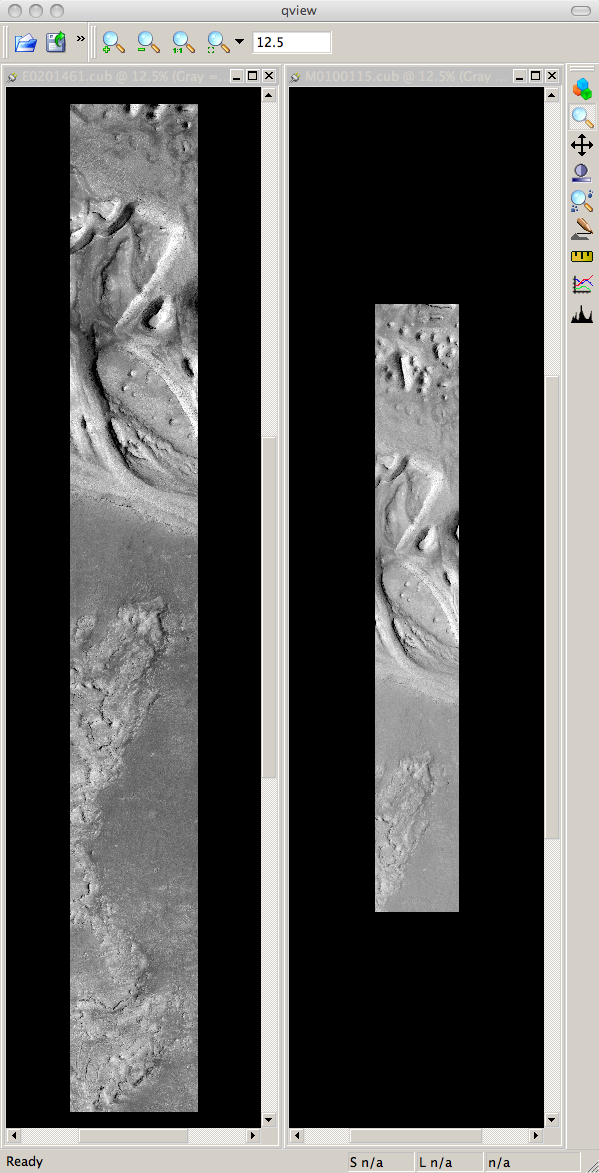
\includegraphics[height=3.7in]{images/p19-images.png}
\hfill
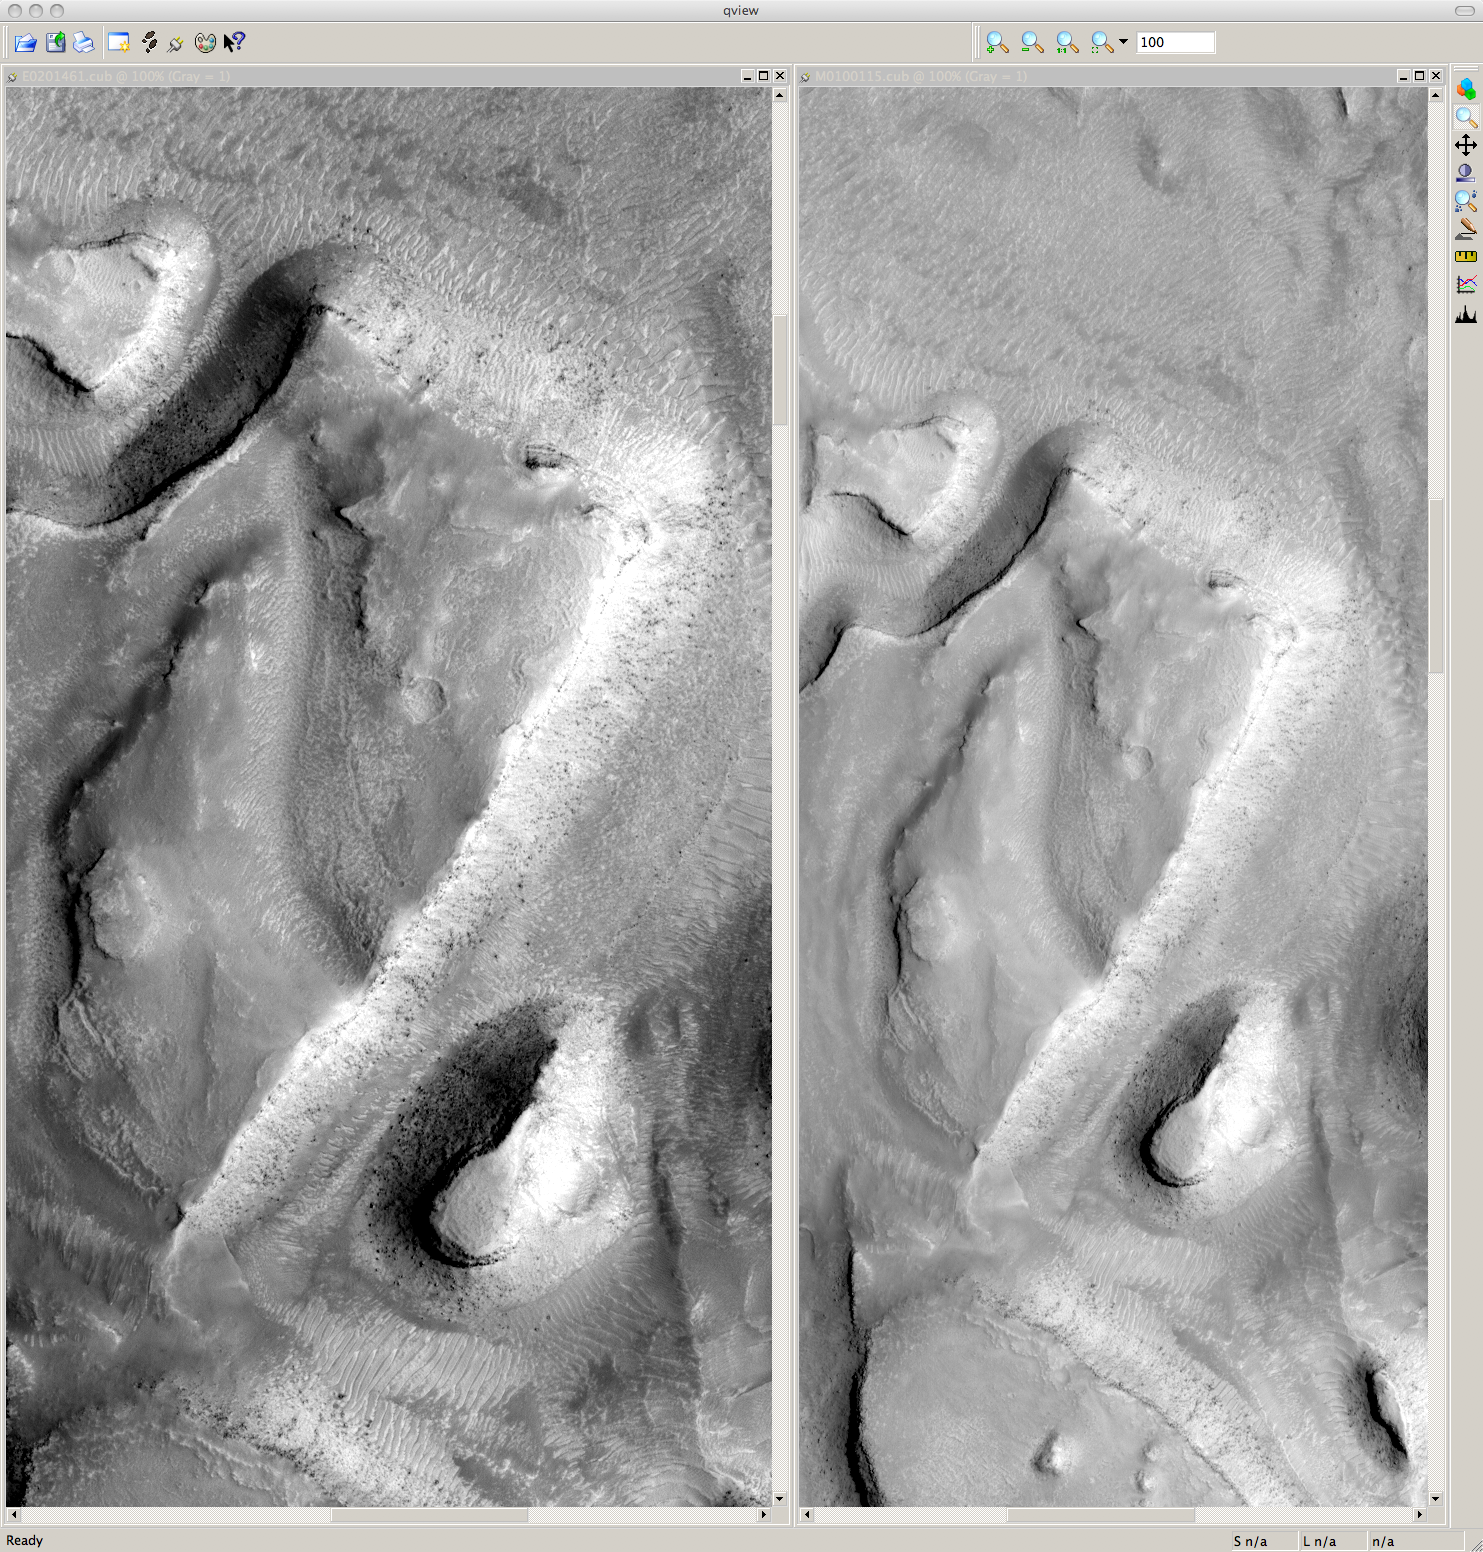
\includegraphics[height=3.7in]{images/p19-images_zoom.png}
\end{minipage}
\hfill
\begin{minipage}{1.3in}
\caption[P19 images open in qview zoomed in]{
    \label{p19-images}
    This shows \texttt{E0201461.cub} and \texttt{M0100115.cub} open in
	ISIS's qview program.  The view on the left shows their full extents
	at the same zoom level, showing how they have different ground scales.
	The view on the right shows them both zoomed in on the same feature.
    }
\end{minipage}
\end{figure}

% \section{Examples of Use}
% 
% Download the tarball and it will unpack into a \texttt{p19} directory.  Create an output directory to hold the results, and invoke the \texttt{stereo} program:
% 
% \begin{verbatim}
% 	mkdir results
% 	stereo E0201461.cub M0100115.cub results/p19
% \end{verbatim}
% 
% You can look at the results by examining the disparity images. These
% show the horizontal and vertical components of the matching offsets
% for each pixel, and they can be a useful debugging tool if you want
% to check how the stereo matcher performed for a given stereo pair:
% 
% \begin{verbatim}
% 	cd results
% 	disparitydebug p19-D.exr -o p19-D     
% 	disparitydebug p19-F.exr -o p19-F
% \end{verbatim}
% 
% \emph{MJB: What exactly is being examined in the resultant images, what are users looking for?}
% 
% A 3D mesh can be built from the point cloud and viewed using the
% \texttt{osgviewer} program:
% 
% \begin{verbatim}
% 	point2mesh p19-PC.tif p19-L.tif -o p19
% 	osgviewer p19.ive
% \end{verbatim}
% 
% When the \texttt{osgviewer} starts, you may want to turn off the
% lighting (hit the `L' key).
% 
% A gridded DEM with floating point pixels can also be built from the point cloud:
% 
% \begin{verbatim}
% 	point2dem --xyz-to-lonlat -r mars p19-PC.tif -n -o p19
% \end{verbatim}
% 
% You can also orthoproject the raw satellite imagery onto the DEM during this step:
% 
% \begin{verbatim}
% 	point2dem --xyz-to-lonlat -r mars p19-PC.tif -o p19 --orthoimage p19-L.tif
% \end{verbatim}
% 
% Finally, you can create colorized, shaded relief (or both) images from the DEM, using these Vision Workbench programs:
% 
% \begin{verbatim}
% 	colormap p19-DEM.tif -o p19-colorized.tif
% 	hillshade p19-DEM.tif -o p19-shaded.tif -e 25
% 	colormap p19-DEM.tif --shaded-relief-file p19-shaded.tif -o p19-color-shaded.tif
% \end{verbatim}
% 
% Finally, you can run the Vision Workbench's \texttt{image2qtree} on any of the following files:
% 
% \begin{itemize}
% \item p19-DEM-normalized.tif
% \item p19-DRG.tif 
% \item p19-shaded.tif
% \item p19-colorized.tif
% \item p19-shaded-colorized.tif
% \end{itemize}


\section{Tutorial}

The following example will utilize images from the example MOC
dataset, discussed above.  The two example ISIS 3 image files are
\texttt{E0201461.cub} and \texttt{M0100115.cub}.

The \texttt{stereo} program (page \pageref{stereo}) is designed for
automated tie point matching and stereo production, and is the first
Stereo Pipeline tool we'll use.

If you like, you should create a directory for the results of the
processing.  The \texttt{stereo} program can generate a number of
output files, and we find it helpful to put them all in a directory,
but it isn't required.

\begin{verbatim}
    > ls
    E0201461.cub   M0100115.cub
    > mkdir results
\end{verbatim}
\noindent
The \texttt{stereo} program requires a \texttt{stereo.default} file
which can be altered for your needs.  Its contents are detailed on
page \pageref{stereo.default}.  You may find it useful to save
multiple versions of the \texttt{stereo.default} file for various
processing needs. If you need to do that, be sure to specify which
configuration file \texttt{stereo} should use with the \texttt{-s}
option.  If this option is not given, the \texttt{stereo} program
will search for a file named \texttt{stereo.default} in the current
directory and will complain if there isn't one.

Then run \texttt{stereo} like this (there should be a
\texttt{stereo.default} file distributed along with the example
data set):

\begin{verbatim}
    stereo E0201461.cub M0100115.cub results/E0201461-M0100115
\end{verbatim}
\noindent
So that last text can be anything you want it to be.  It designates
the text that \texttt{stereo} will use as a prefix for its many
output files.  Since the first part is \texttt{results/} this causes
the program to put the results in that directory with files whose
names start with \texttt{E0201461-M0100115}.  If instead that last
text was just \texttt{E0201461-M0100115} it would have created a
bunch of files that start with \texttt{E0201461-M0100115} in the
same directory as the input files.

The \texttt{stereo} program's processing moves through several
stages which are detailed on page \pageref{entrypoints}.  However,
once the \texttt{stereo} program completes, it creates a number of
files.  A quick look at some of the TIFF files created, can quickly
give you an idea of what the \texttt{stereo} program did (figure
\ref{p19-stereo-output}).


\begin{figure}
\begin{center}
\includegraphics[width=5in]{images/p19-stereo-output.png}
\caption[P19 stereo output images]{
    \label{p19-stereo-output}
	These are the four viewable \texttt{.tif} files created by
	the \texttt{stereo} program.  The left two are the aligned
	images (\texttt{E0201461-M0100115-L.tif} and
	\texttt{E0201461-M0100115-R.tif}).  The next two images are
	the mask images (\texttt{E0201461-M0100115-lMask.tif} and
	\texttt{E0201461-M0100115-rMask.tif}), which indicate which
	pixels in the aligned images are good to use for the next
	step.  The image on the right is the Good Pixel map
	(\texttt{E0201461-M0100115-GoodPixelMap.tif}), which indicates
	the pixels in grey which were successfully matched with the
	correlator.  The red pixels were not.  Those red pixels which 
	are not black in both mask images are optionally filled later
	during the hole-filling step.
    }
\end{center}
\end{figure}

% \begin{figure}
% \begin{center}
% 
\includegraphics[height=8in]{images/p19-goodpixel.png}
% \caption[P19 good pixel image]{
%     \label{p19-goodpixel}
% 	The Good Pixel map. 
% 	Red pixels are not useful for alignment. 
%     }
% \end{center}
% \end{figure}
% 
% \begin{figure}
% \begin{center}
% 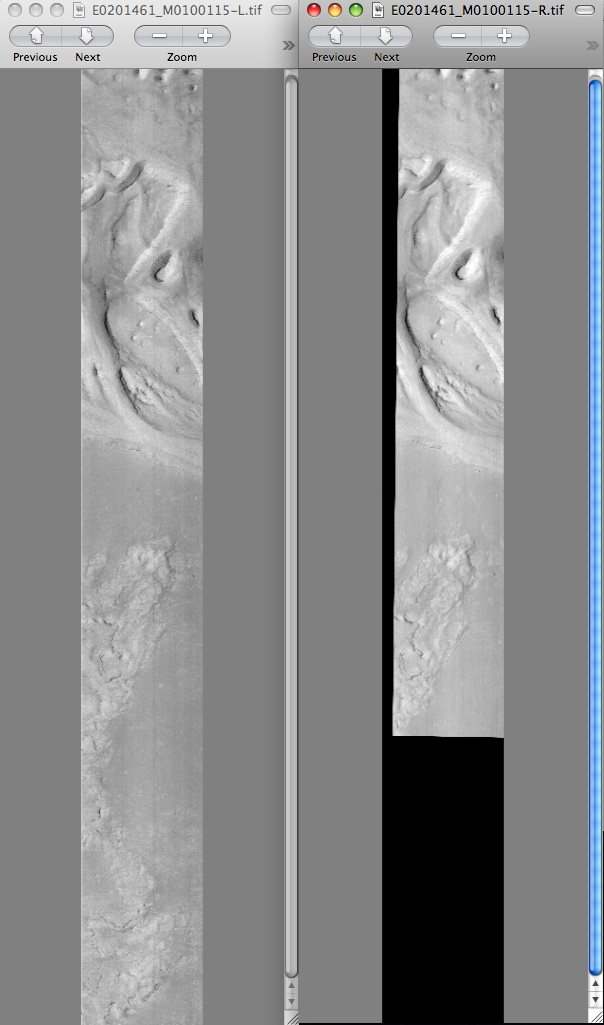
\includegraphics[width=3in]{images/p19-aligned.png}
% \caption[P19 aligned image]{
%     \label{p19-aligned}
% 	The left and right aligned images.
%     }
% \end{center}
% \end{figure}

If the above TIFF files look okay, you can probably just go on to
making a mesh or a DTM from the point cloud file
(\texttt{E0201461-M0100115-PC.tif}).  However, to get an idea of the
disparity information that the \texttt{stereo} program created and then
used to build the point cloud, it can be useful to take a look at that
disparity information.  The \texttt{stereo} program records this information
in the \texttt{E0201461-M0100115-D.exr} file.

To begin an examination of the results, you must first examine the
disparity images. These images show the horizontal and vertical
components of the matching offsets for each pixel. They are
particularly useful if you want to check the performance of the
stereo matcher for any given stereo pair and they can be used as a
debugging tool.

Move into the directory that contains your results, and run the
\texttt{disparitydebug} program (page \pageref{disparitydebug}) to
examine the disparity files.

\begin{verbatim}
    cd results
    disparitydebug p19-D.exr -o p19-D     
    disparitydebug p19-F.exr -o p19-F
\end{verbatim}

\emph{MJB: What exactly is being examined in the resultant images, what are users looking for?  What are the probable failure scenarios?  Discuss them and potential remedies.}


\begin{figure}
\begin{center}
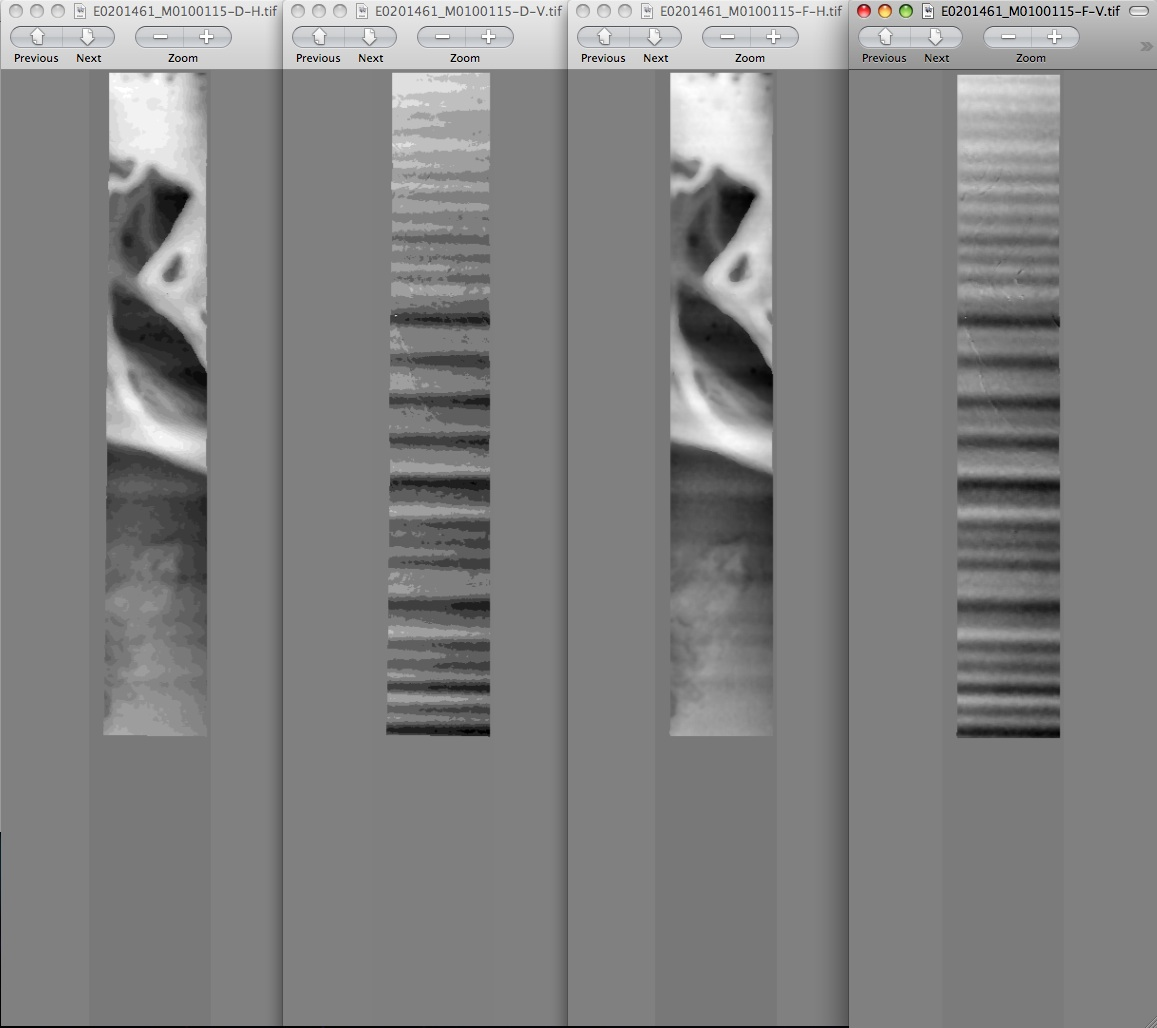
\includegraphics[width=4in]{images/p19-disparity.png}
\caption[P19 disparity images]{
    \label{p19-disparity}
	The disparity images.
    }
\end{center}
\end{figure}

The next step is to produce a 3D mesh with \texttt{point2mesh} (page
\pageref{point2mesh}).  This image can be viewed with \texttt{osgviewer}
(the Open Scene Graph Viewer program, distributed with the binary version
of the Stereo Pipeline).  The \texttt{point2mesh} program takes the
point cloud file and one of the image files (usually the highest
resolution one) created by \texttt{stereo} as inputs.

\begin{verbatim}
    point2mesh p19-PC.tif p19-L.tif -o p19
\end{verbatim}

This will create the file \texttt{p19.ive}, openable with the
\texttt{osgviewer}. When the \texttt{osgviewer} starts, you may
want to turn off the lighting (hit the `L' key).

The \texttt{point2dem} program (page \pageref{point2dem}) creates
a digital elevation model (DEM) from the Point Cloud file.

\begin{verbatim}
    point2dem p19-PC.tif -o p19
\end{verbatim}

The resultant file ...

You can specify a coordinate system (e.g., latlon) and a reference
spheroid (i.e., calculated for the Moon or Mars). You also have the
option of creating a normalized DEM in addition to the automatically
generated non-normalized DEM.


\begin{verbatim}
    point2dem --xyz-to-lonlat -r mars p19-PC.tif -n -o p19
\end{verbatim}

The \texttt{point2dem} program can also be used to orthoproject raw
satellite imagery onto the DEM. To do this, invoke \texttt{point2dem}
just as before, but add the \texttt{orthoimage} option and specify
the use of the Left image file as the texture file to use for the
projection.

\begin{verbatim}
    point2dem --xyz-to-lonlat -r mars p19-PC.tif -o p19 --orthoimage p19-L.tif 
\end{verbatim}

The \texttt{point2dem} program can be used in many different ways.
Be sure to explore all of the options.

\begin{figure}
\begin{center}
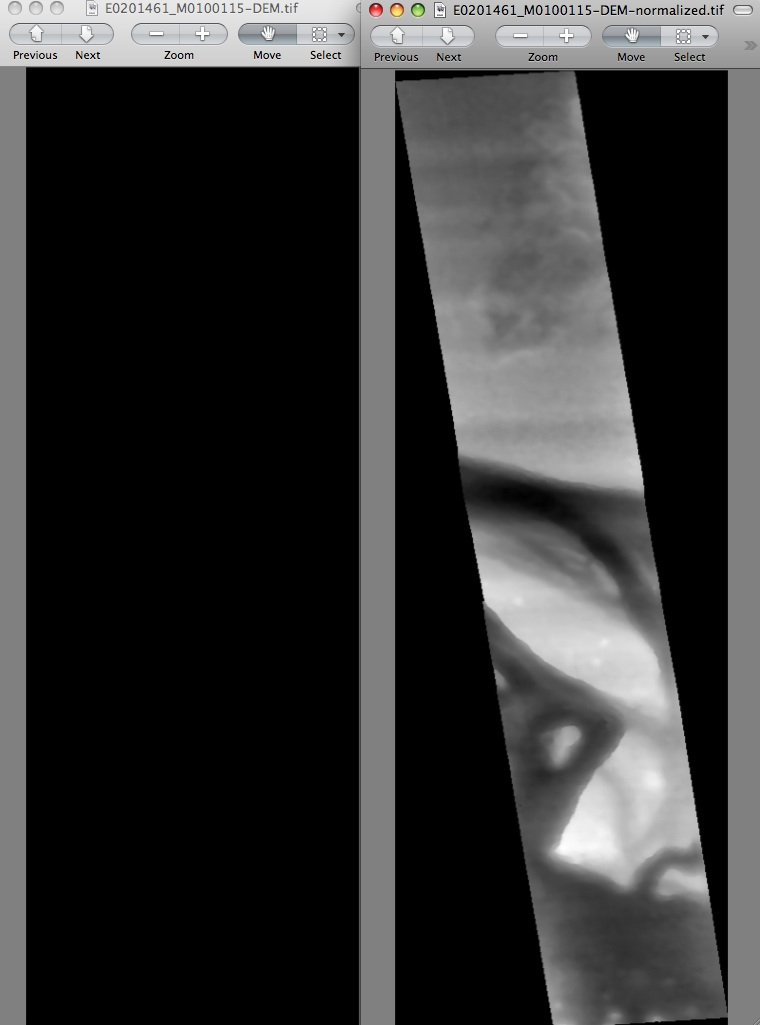
\includegraphics[width=4in]{images/p19-dems.png}
\caption[P19 dem images]{
    \label{p19-dems}
	The non-normalized and normalized DEMs. Note that the
	non-normalized version contains floating point pixel values
	and will not open in most image viewing programs which
	expect integer pixel values between 0 and 255 (which is
	what the normalized version does for you).
    }
\end{center}
\end{figure}

\begin{figure}
\begin{center}
\includegraphics[width=3in]{images/p19-ortho.png}
\caption[P19 orthophoto]{
    \label{p19-ortho}
	The left image orthoprojected onto the DEM.
    }
\end{center}
\end{figure}

Once you have generated a DEM, you can use the Vision Workbench's
\texttt{colormap} and \texttt{hillshade} tools to create colorized
and/or shaded relief images from the DEM.

To create a colorized version of the DEM, you need only specify the
DEM file to use:

\begin{verbatim}
    colormap p19-DEM.tif -o p19-colorized.tif
\end{verbatim}

To create a hillshade of the DEM, you should specify the DEM file
to use. It is also advisable to explore the effects of altering the
elevation of the light source.

\begin{verbatim}
    hillshade p19-DEM.tif -o p19-shaded.tif -e 25
\end{verbatim}

To create a colorized version of the shaded relief file, specify
the DEM and the shaded relief file that should be used.

\begin{verbatim}
    colormap p19-DEM.tif --shaded-relief-file p19-shaded.tif -o p19-color-shaded.tif
\end{verbatim}

\begin{figure}
\begin{center}
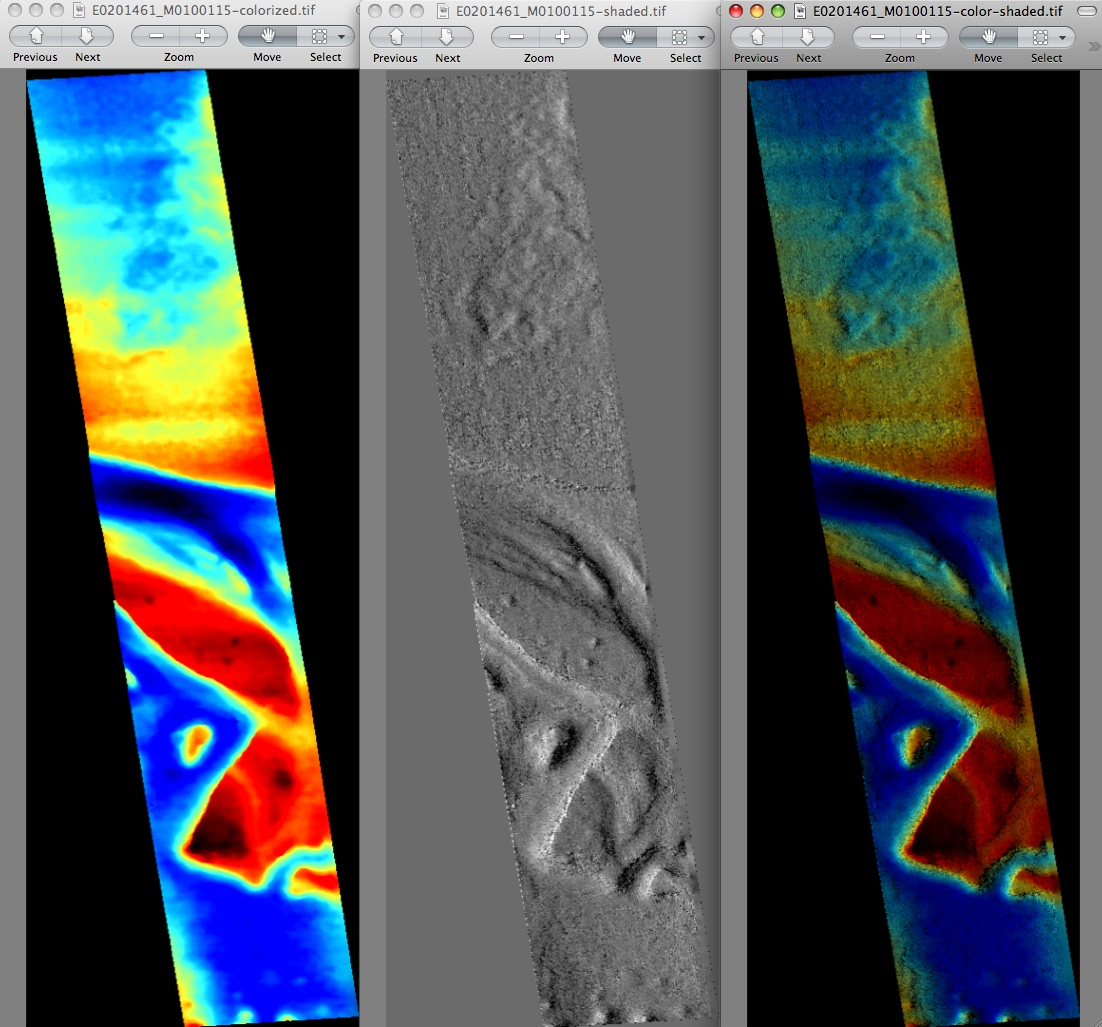
\includegraphics[width=5in]{images/p19-colorized-shaded.png}
\caption[P19 colorized and shaded relief]{
    \label{p19-color}
	The colorized DEM, the shaded relief image, and the colorized hillshade.
    }
\end{center}
\end{figure}

The final option of the stereo processing package is \texttt{image2qtree}.
This function was designed for use in creating geographically
referenced images in tiles such that each tile can be viewed at
ideal resolution.

The \texttt{image2qtree} program can be used on any of the following files that you 
have generated:
\begin{verbatim}
    p19-DEM-normalized.tif
    p19-DRG.tif 
    p19-shaded.tif
    p19-colorized.tif
    p19-shaded-colorized.tif
\end{verbatim}

Specify which image you would like to invoke \texttt{image2qtree} on, along
with any combination of options.

\begin{verbatim}
    image2qtree p19-DEM-normalized.tif -o p19-DEM-n-qtree
\end{verbatim}


